\subsection{Registrering på PDF}
I dette afsnit vises design, bruger grænseflade, implementering og test for 'Registrering på PDF' viewet. For den fulde dokumentation henvises til Arkitektur og Design dokumentationens afsnit \ref{Design-sec:PDF}.
\subsubsection{Design}
Sekvensdiagrammerne for registrering på PDF tegning, er opdelt i tre for at overskueligegøre flowet. \\
Det første sekvensdiagram viser hvordan applikationen loader PDF tegningen ind. Sekvensdiagrammet kan ses på figur \ref{fig:LoadPDFSekvensDiagram}.
\begin{figure}[H] % (alternativt [H])
	\centering
	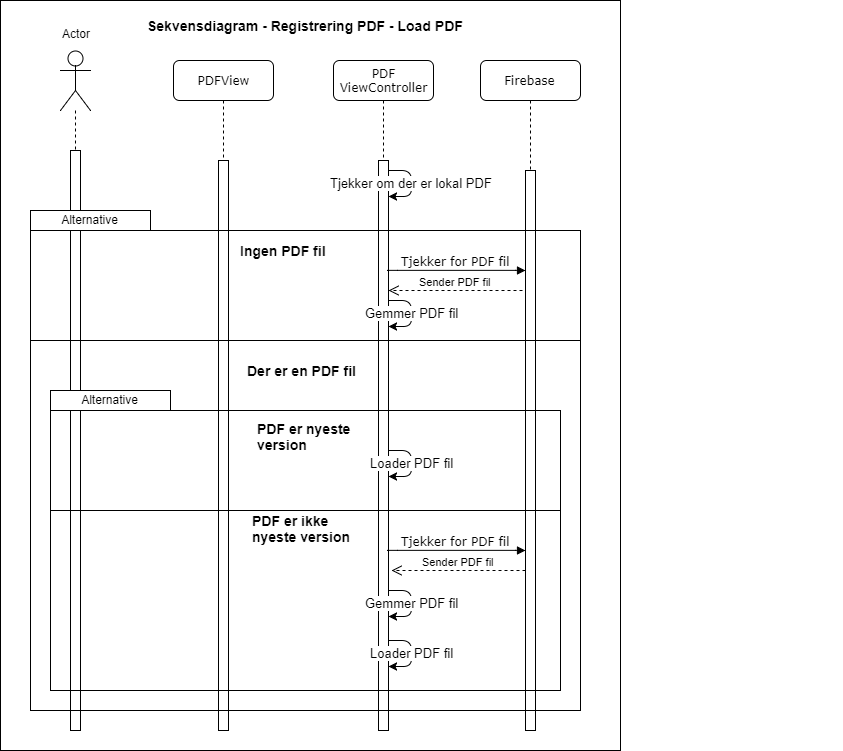
\includegraphics[height=12cm, width=15cm]{Design/Applikation/RegistrePDF/LoadPDFSekvensDiagram}
	\caption{Sekvensdiagram for Registrering på PDF - Loading af PDF, i Rambøll Tilsyn.}
	\label{fig:LoadPDFSekvensDiagram}
\end{figure}

\clearpage

Andet sekvensdiagram iser hvordan JSON filen bliver oprettet. Sekvensen med JSON sker direkte efter at PDF sekvensen er overstået. Sekvensdiagrammet kan ses på figur \ref{fig:LoadJSONSekvensDiagram}.
\begin{figure}[H] % (alternativt [H])
	\centering
	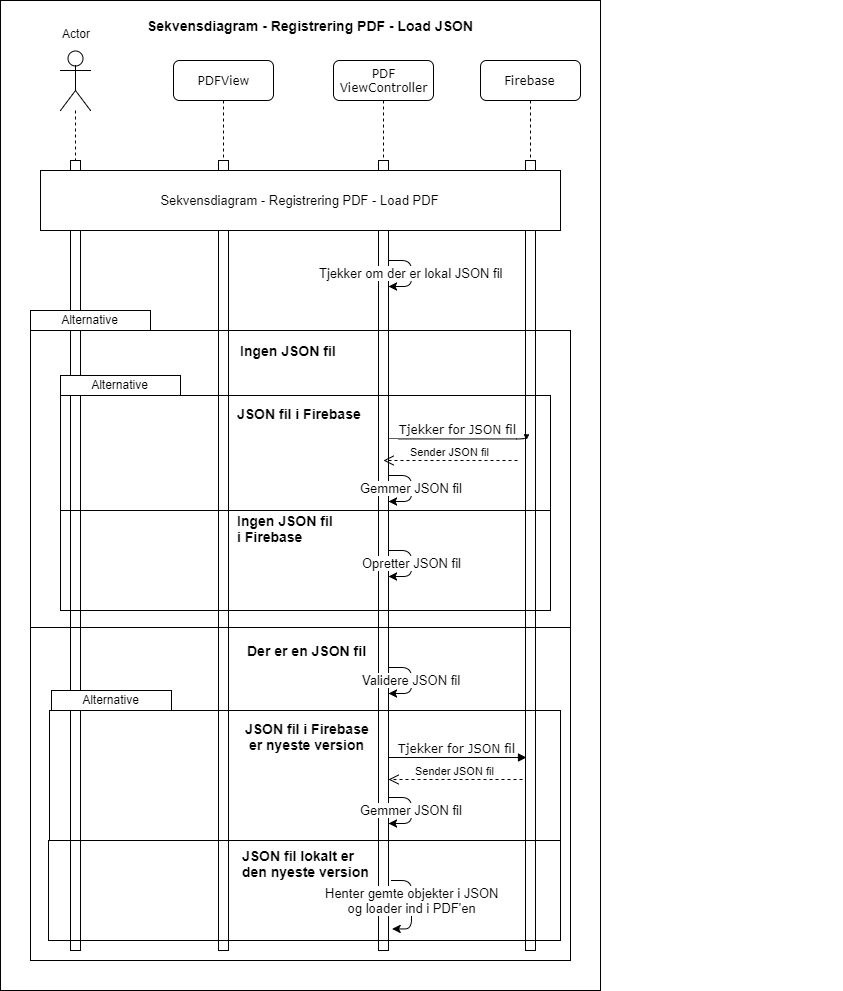
\includegraphics[height=15cm, width=15cm]{Design/Applikation/RegistrePDF/LoadJSONSekvensDiagram}
	\caption{Sekvensdiagram for Registrering på PDF - Loading af JSON, i Rambøll Tilsyn.}
	\label{fig:LoadJSONSekvensDiagram}
\end{figure}

\clearpage

Sidste sekvensdiagram, som sker i forlængelse af først Loading af PDF og Load JSON, viser hvordan systemet agere, når brugeren interagere med applikationen i forbindelse med oprettelse af objekter på PDF tegningen. Sekvensdiagrammet for dette kan ses på \ref{fig:RegistrerObjekterSekvensDiagram}.
\begin{figure}[H] % (alternativt [H])
	\centering
	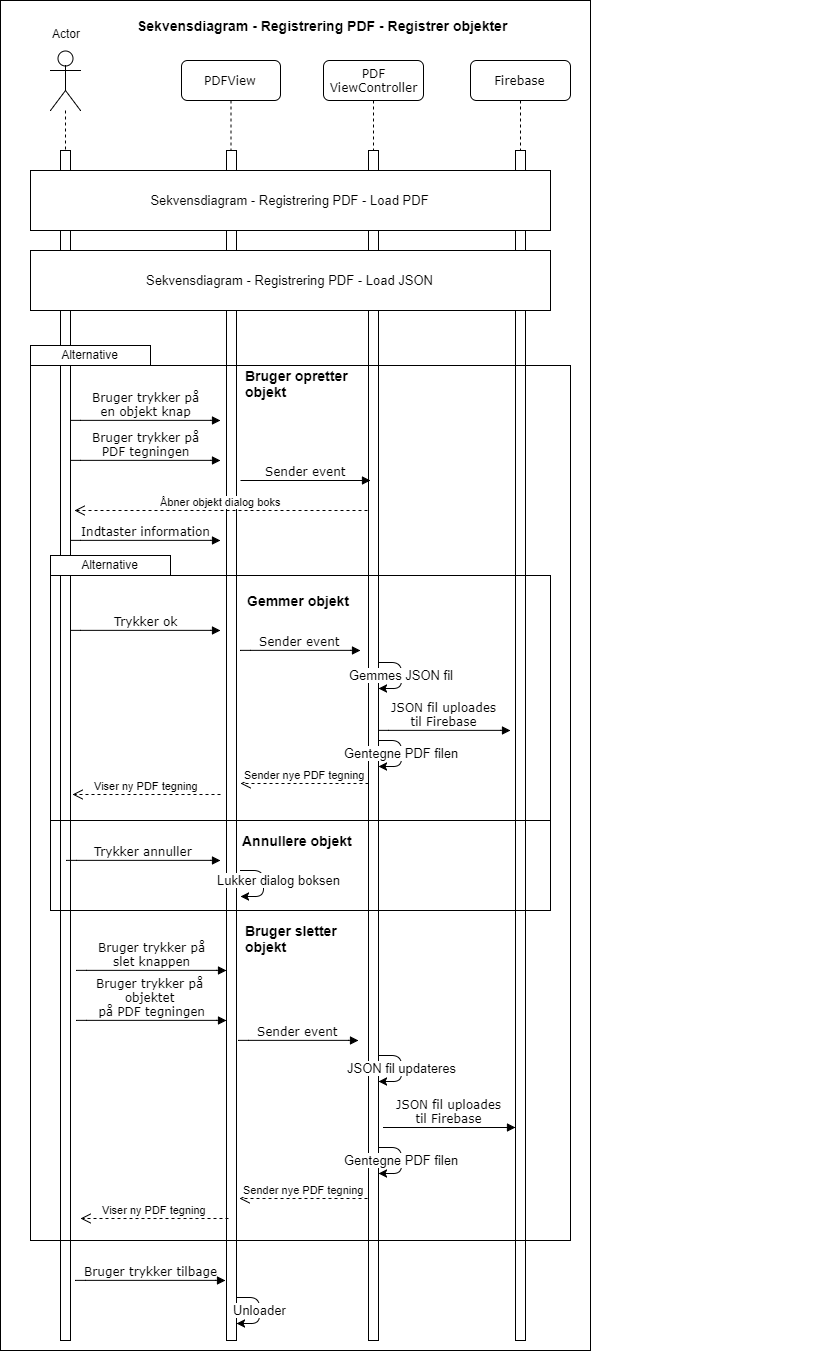
\includegraphics[height=18cm, width=15cm]{Design/Applikation/RegistrePDF/RegistrerObjekterSekvensDiagram}
	\caption{Sekvensdiagram for Registrering på PDF - Registrer på PDF, i Rambøll Tilsyn.}
	\label{fig:RegistrerObjekterSekvensDiagram}
\end{figure}

\clearpage

\subsubsection{Grafisk brugergrænseflade}
Grænsefladen for 'Registrer på PDF' viewet som ses på figur \ref{fig:RegistrerObjekterView} består af to views. 
Det øverste view viser PDF'en som tilhører projektet. \\
Det nederste view indeholder knapper som brugeren kan interagere med. Der er seks forskellige knapper: \\
De første to er frem og tilbage, hvor brugeren kan bladre mellem de forskellige sider i PDF'en. De tre knapper der kommer efter, er de symboler som brugeren kan tegne på PDF'en, ved at trykke på knappen og derefter det sted på PDF'en han ønsker. \\
Sidste knap er en liste knap. Her har brugeren mulighed for at afslutte sin registrering.
\begin{figure}[H] % (alternativt [H])
	\centering
	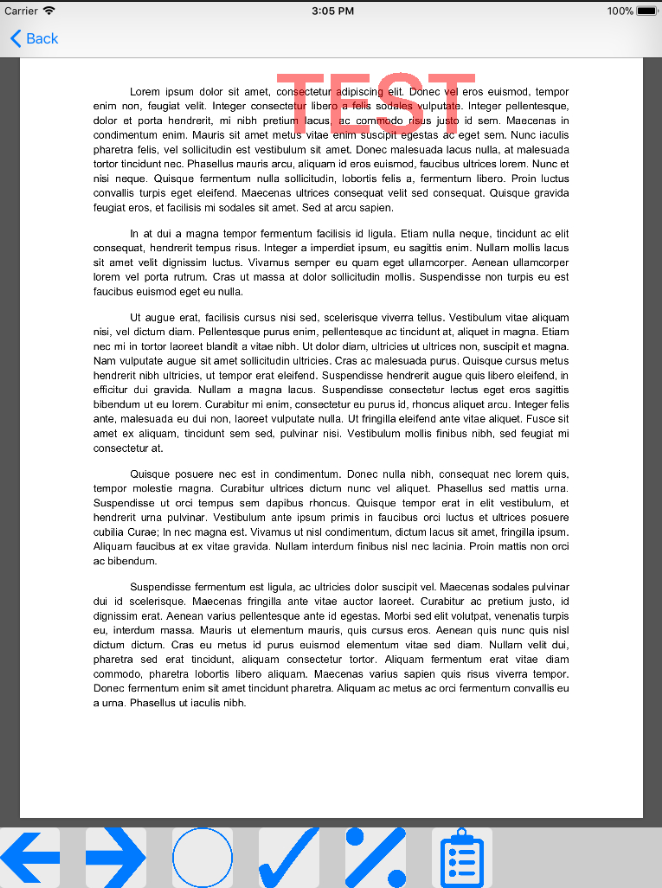
\includegraphics[height=18cm, width=15cm]{Design/Applikation/RegistrePDF/PDF}
	\caption{Registrer på PDF viewet som det er implementeret i Rambøll Tilsyn.}
	\label{fig:RegistrerObjekterView}
\end{figure}

\subsubsection{Implementering}

\subsubsection{Test}

\clearpage